% Intestazione
\fancyhead[L]{4 \hspace{0.2cm} Guida all’utilizzo} % Testo a sinistra 

\section{Guida all’utilizzo}
\label{sec:guida_utilizzo}


\subsection{Cosa chiedere, e come chiederlo}
\label{subsec:cosa_come_chiedere}

BuddyBot è pensato per essere l'assistente digitale di un'azienda informatica che desidera aiutare i propri dipendenti a ricercare in
modo efficiente ed efficace le informazioni di interesse nel codice e nella documentazione dei vari progetti aziendali. Più precisamente, ad
ogni interrogazione posta dall'utente vengono associati
dei documenti di contesto, che provengono esclusivamente dai profili \emph{GitHub}\textsubscript{\textbf{\textit{G}}},
\emph{Jira}\textsubscript{\textbf{\textit{G}}} e \emph{Confluence}\textsubscript{\textbf{\textit{G}}} dell'azienda, e, in base alle
informazioni presenti su tali documenti di contesto, il chatbot fornirà la risposta alla domanda ricevuta.
Se la domanda viene malposta, il chatbot potrebbe non essere in grado di fornire una risposta, e in tal caso potrebbe restituire
uno dei seguenti messaggi:
\begin{itemize}
    \item \emph{"Domanda fuori contesto"}: la domanda posta non è inerente al contesto informatico aziendale;
    \item \emph{"Informazione non trovata"}: non è stato possibile trovare nei documenti di contesto informazioni utili per rispondere
    alla domanda.
\end{itemize}

E' tuttavia possibile che il chatbot restituisca tali risposte anche in casi in cui non ce lo si aspetta.
Per evitare di ottenere risposte negative, forniamo qui di seguito delle istruzioni per capire come porre la domanda per
ottenere una risposta soddisfacente:
\begin{enumerate}
    \item La domanda deve essere concisa e diretta, senza giri di parole. Ad esempio "Qual è lo stato del progetto X su Jira?" invece
    che "Potresti gentilmente dirmi qual è lo stato attuale del progetto X su Jira, per favore?";
    \item Si devono mettere bene in risalto le parole chiave. Ad esempio "Qual è l'errore di build nel progetto Y?" invece che "Qual
    è il problema con il progetto Y?";
    \item La domanda deve essere il più breve possibile. Ad esempio "Chi è l'assegnatario del ticket Z?" invece che "Vorrei sapere
    chi è la persona a cui è stato assegnato il ticket Z";
    \item La domanda deve essere pensata per ottenere una risposta unitaria, e non per aprire una discussione. Ad esempio, occorre
    unificare "Quali commit sono stati fatti oggi? Mostrameli in forma di tabella con assegnatario e data" invece che porre due domande
    separate "Quali commit sono stati fatti oggi?" e "Mostrameli in forma di tabella con assegnatario e data", perchè in quest'ultimo
    caso la seconda domanda riceverà come risposta "Domanda fuori contesto": infatti, ogni coppia domanda-risposta è a sè stante, cioè
    il chatbot non considera il completo flusso del discorso per generare la risposta all'interrogazione corrente, bensì considera solo
    quest'ultima. Le domande suggerite per proseguire sono infatti pensate per guidare l'utente verso una nuova interrogazione correlata alla precedente, e non per far
    completare la risposta alla domanda corrente;
    \item La domanda deve riguardare un contesto chiaro e definito, quindi non può toccare tematiche troppo generali. Ad esempio
    "Quali sono i task aperti per il progetto A?" invece che "Qual è la situazione dei nostri progetti?";
    \item Il suddetto contesto deve essere uno, infatti non si possono porre due o più domande a tema differente in una stessa
    interrogazione. Ad esempio, invece che "Chi è l'assegnatario del ticket Z su Jira
    e quali sono i suoi relativi commit su GitHub?", è meglio separare in "Chi è l'assegnatario del ticket Z su Jira?" e poi, una 
    volta ricevuta la risposta, "Quali sono i commit di persona Y su GitHub?" (specificando chiaramente la persona, poichè, come suddetto, il chatbot non può visualizzare il messaggio precedente);
    \item Non si devono chiedere informazioni generiche a riguardo di una risorsa fornendo solo il nome della stessa, ma bisogna
    bensì specificare più di preciso cosa si vuole sapere a riguardo di tale risorsa. Ad esempio "Qual è la descrizione del ticket
    Z su Jira?" invece che "Dimmi qualcosa sul ticket Z";
    \item La domanda deve essere posta in un linguaggio quanto più possibile formale e tecnico, cercando di rimanere aderenti
    allo stile di scrittura dei documenti aziendali. Un linguaggio troppo colloquiale quasi sicuramente condurrà a risposte negative.
    Ad esempio "Qual è la copertura dei test per il modulo B?" invece che "Come stanno andando i test per il modulo B?";
    \item Non si devono porre domande che richiedono una risposta soggettiva. In caso ne venga posta una per sbaglio, non ci si deve
    fidare della risposta fornita, è bensì consigliabile chiedere ad un collega. Ad esempio "A quanto ammonta la copertura del codice
    nel progetto C?" invece che "Pensi che il codice del progetto C sia buono?";
    \item Si devono evitare domande che richiedano ragionamento e/o collegamenti logici, in quanto il chatbot non è in grado di
    processare informazioni in tal senso. Ad esempio "Quali sono i commit svolti tra il 6 ed il 10 febbraio nel progetto D?" invece che "Quali sono i
    commit svolti nel progetto D dall'inizio della sprint ad ora?";
    \item Non si devono porre domande per la cui risposta è necessaria una ricerca su internet, in quanto il chatbot fa
    riferimento esclusivamente ai documenti di contesto, e non è abile a ricavare informazioni attendibili in rete. Ad esempio, invece che "Nel
    progetto Y viene utilizzata l'ultima versione rilasciata del framework X?", bisogna chiedere "Qual è la versione del framework X
    che viene utilizzata nel progetto Y?" e poi cercare manualmente su internet se tale versione è l'ultima rilasciata o meno.
\end{enumerate}

\newpage


\subsection{Interrogazione del chatbot}

\subsubsection{Come inserire una domanda}  
\label{subsec:come_inserire_domanda}  

Una volta aperta l'applicazione, è possibile inserire una domanda scrivendo liberamente nella barra di input, in qualsiasi momento della conversazione.\\
A partire dalla seconda interrogazione, oltre alla possibilità di scrivere liberamente, vengono proposti tre suggerimenti selezionabili per facilitare la continuazione del dialogo.\\
Questi suggerimenti sono opzionali e possono essere utilizzati per proseguire più rapidamente la conversazione, o ignorati in favore di un messaggio personalizzato.\\
La domanda va scritta nella barra di input dove appare il testo \textit{Scrivi un messaggio...}. Quando si posiziona il cursore e si clicca nel campo per iniziare a scrivere, il bordo del campo diventa blu, indicando che è pronto per ricevere il testo.\\
Il pulsante "Invia", situato a destra della barra di input, è disattivato e di colore grigio quando la barra è vuota. Non appena si inizia a scrivere, il pulsante si attiva e diventa blu.
Il messaggio può essere inviato sia cliccando sul pulsante "Invia" che premendo il tasto \textit{Enter} sulla tastiera.\\
Di seguito sono elencate le configurazioni dei componenti di input in alcune situazioni:

\begin{itemize}  
    \item \textbf{Scrittura libera - campo vuoto}: Quando il campo è vuoto, il pulsante "Invia" è disattivato e grigio, poichè non è possibile inviare un messaggio fino a quando non viene scritto del testo, come mostrato in figura \bulref{fig:Barra per l'invio di una domanda libera vuota};
    \item \textbf{Scrittura libera - campo pieno}: Quando il campo contiene del testo, il pulsante "Invia" diventa attivo e blu, come mostrato in figura \bulref{fig:Barra per l'invio di una domanda libera piena};
    \item \textbf{Caricamento dopo l'invio di una domanda}: Quando viene cliccato il pulsante "Invia" oppure il tasto "Enter", il messaggio viene visualizzato sul lato destro della schermata, mentre, sul lato sinistro, compare un'icona di una banana morsicata che rotea su se stessa, indicando che il messaggio è in fase di elaborazione, come mostrato in figura \bulref{fig:Icona di caricamento dopo l'invio di una domanda}. La barra di input e il pulsante "Invia" vengono disabilitati durante questo processo, per impedire la scrittura e l'invio di ulteriori messaggi fino a quando non viene visualizzata la risposta;
    \item \textbf{Suggerimenti - campo vuoto}: Dalla seconda interrogazione in poi, tre suggerimenti vengono proposti sopra la barra di input per facilitare la continuazione della conversazione. Subito dopo l'invio del messaggio, la barra di input si svuota e il pulsante "Invia" viene disattivato, come mostrato in figura \bulref{fig:Domande per proseguire la conversazione con barra vuota};
    \item \textbf{Suggerimenti - campo pieno}: Dalla seconda interrogazione in poi, pur avendo disponibili i tre suggerimenti, è ancora possibile inserire una domanda libera nella barra di input. Se la barra contiene testo, il pulsante "Invia" è attivo e blu, come mostrato in figura \bulref{fig:Domande per proseguire la conversazione con barra piena}.
\end{itemize}

\begin{figure}[h]
    \centering
        
\includegraphics[width=.8\linewidth]{Barra per l'invio di una domanda libera vuota.png}
        \caption{Barra per l'invio di una domanda libera vuota}
        \label{fig:Barra per l'invio di una domanda libera vuota}        
\end{figure}
\begin{figure}[h]
    \centering
        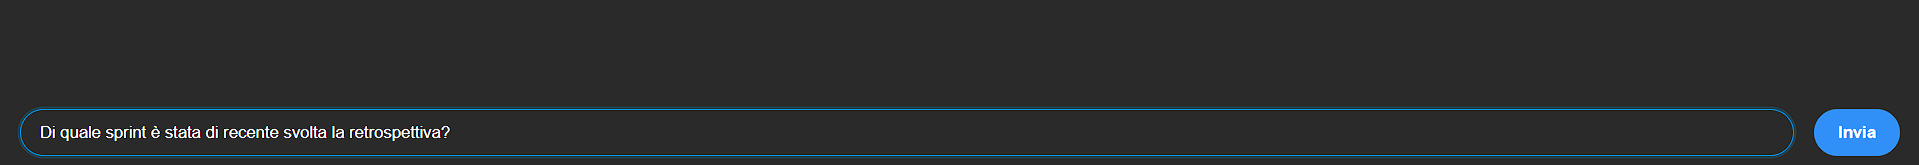
\includegraphics[width=.8\linewidth]{Barra per l'invio di una domanda libera piena.png}
        \caption{Barra per l'invio di una domanda libera piena}
        \label{fig:Barra per l'invio di una domanda libera piena}        
\end{figure}

\newpage

\begin{figure}[h]
    \centering
        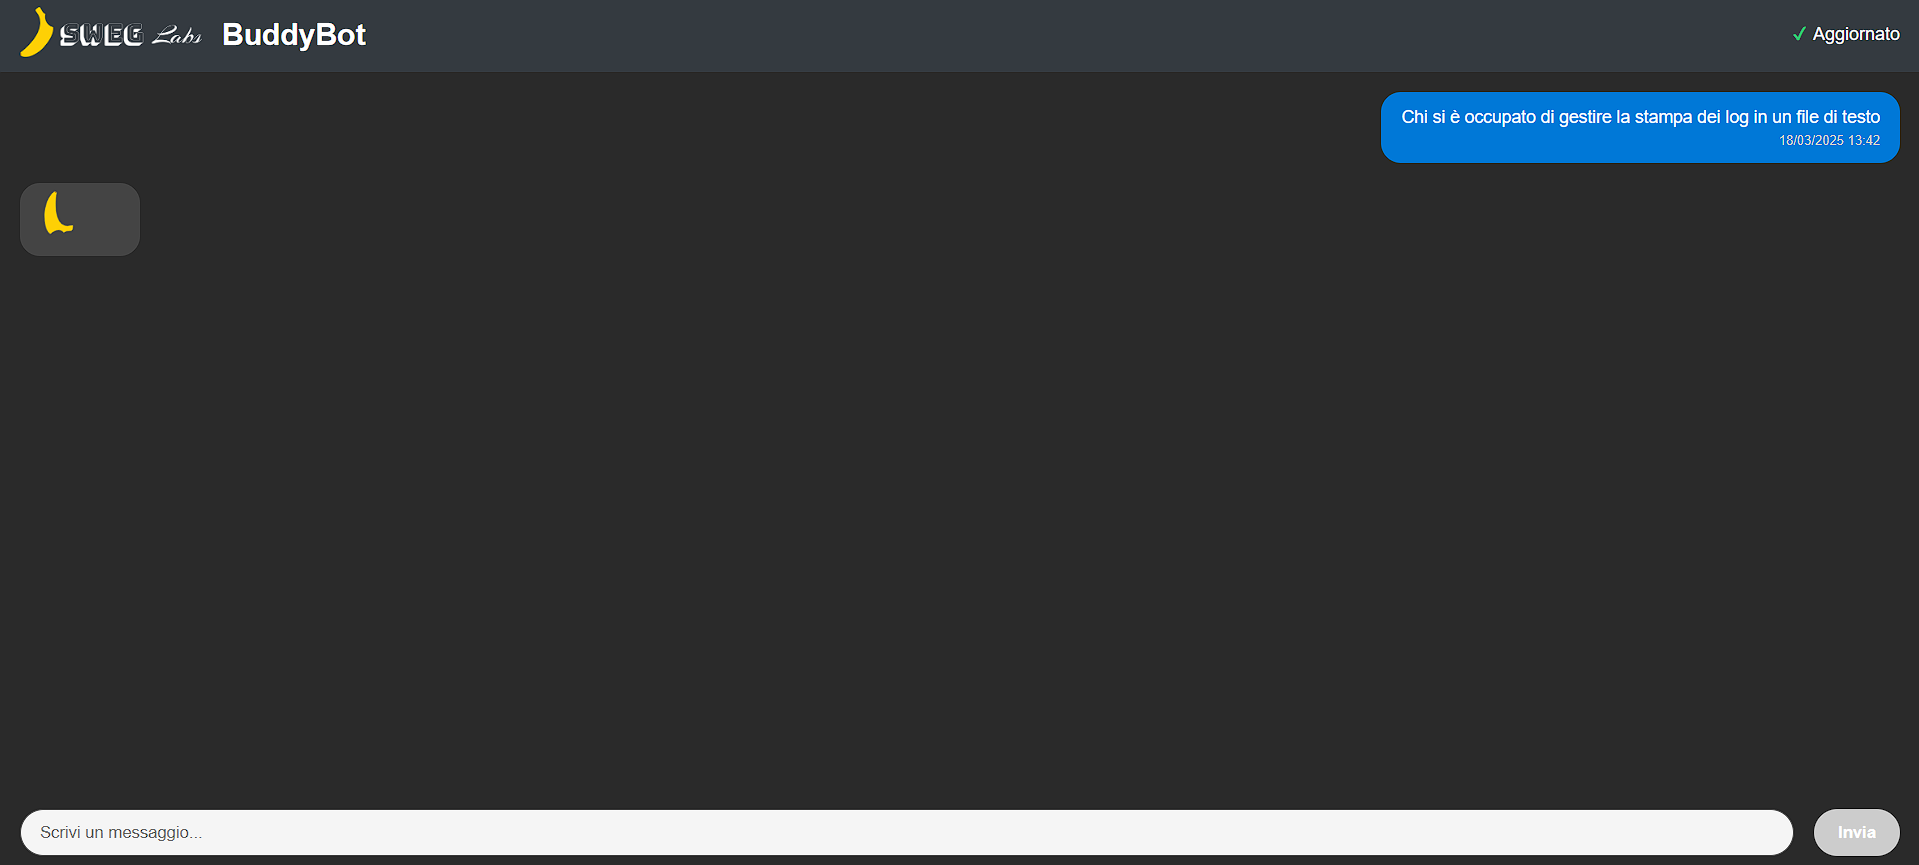
\includegraphics[width=.8\linewidth]{Icona di caricamento dopo l'invio di una domanda.png}
        \caption{Icona di caricamento dopo l'invio di una domanda}
        \label{fig:Icona di caricamento dopo l'invio di una domanda}
\end{figure}
\begin{figure}[h]
    \centering
        
\includegraphics[width=.8\linewidth]{Domande per proseguire la conversazione con barra vuota.png}
        \caption{Domande per proseguire la conversazione con barra vuota}
        \label{fig:Domande per proseguire la conversazione con barra vuota}        
\end{figure}
\begin{figure}[h]
    \centering
        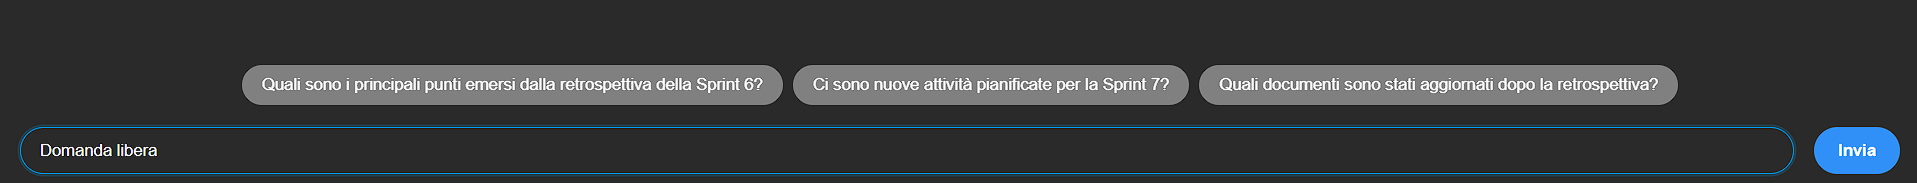
\includegraphics[width=.8\linewidth]{Domande per proseguire la conversazione con barra piena.png}
        \caption{Domande per proseguire la conversazione con barra piena}
        \label{fig:Domande per proseguire la conversazione con barra piena}        
\end{figure}


 
\subsubsection{La risposta del chatbot}  
\label{subsec:la_risposta_del_chatbot}  

Quando il chatbot fornisce una risposta, essa include un testo esplicativo, che talvolta può contenere uno \emph{snippet}\textsubscript{\textbf{\textit{G}}} di codice. Lo snippet viene visualizzato in un riquadro dedicato per facilitare la sua lettura e comprensione.\\
Inoltre, è possibile copiare tramite pulsante sia il messaggio completo che singolarmente gli snippet di codice contenuti nella risposta. Per fare ciò, in alto a destra di ogni messaggio del chatbot e in alto a destra di ogni riquadro di codice, è presente un pulsante dedicato che permette di copiare il contenuto a cui fa riferimento negli appunti. Il pulsante di copia del solo snippet è particolarmente utile quando si desidera utilizzare o condividere direttamente il codice invece che tutta la risposta.\\
I link correlati da cui il chatbot ha ricavato la risposta vengono visualizzati in arancione in un riquadro evidenziato di scuro in fondo alla risposta, permettendo di accedere facilmente alle fonti informative della risposta o ad approfondimenti aggiuntivi. Cliccando su uno di questi link, l'utente verrà indirizzato alla risorsa corrispondente.\\
Gli elementi del messaggio di risposta sono dunque i seguenti:

\begin{itemize}
  \item \textbf{Risposta testuale}: Il chatbot fornisce una risposta testuale che include informazioni esplicative, come mostrato in figura \bulref{fig:Risposta senza snippet di codice};
  \item \textbf{Snippet di codice}: Quando la risposta include uno snippet di codice, questo viene visualizzato all'interno di un riquadro per evidenziarlo chiaramente, come mostrato in figura \bulref{fig:Risposta con snippet di codice};
  \item \textbf{Copia del testo e del codice}: È possibile copiare sia tutto il testo del messaggio che solamente un suo eventuale snippet di codice cliccando sui rispettivi pulsanti di copia situati in alto a destra dell'elemento da copiare, come mostrato in figura \bulref{fig:Pulsante di copia messaggio e pulsante di copia snippet di codice};
  \item \textbf{Link correlati}: I link correlati da cui il chatbot ha ricavato la risposta vengono visualizzati in arancione in un riquadro evidenziato di scuro in fondo alla risposta, e su di essi è possibile cliccare per aprirli ed accedere ad ulteriori risorse, come mostrato in figura \bulref{fig:Riquadro dei link correlati}.
\end{itemize}

\newpage
\begin{figure}[h]
    \centering
        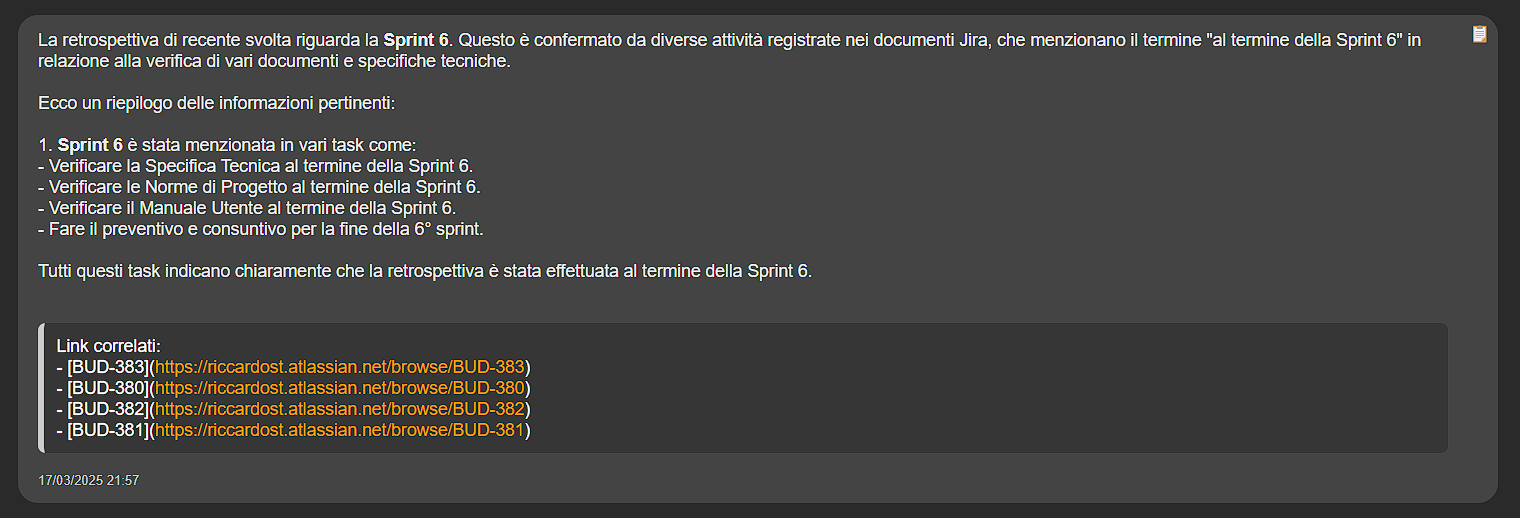
\includegraphics[width=.8\linewidth]{Risposta senza snippet di codice.png}
        \caption{Risposta senza snippet di codice}
        \label{fig:Risposta senza snippet di codice}        
\end{figure}
\begin{figure}[h]
    \centering
        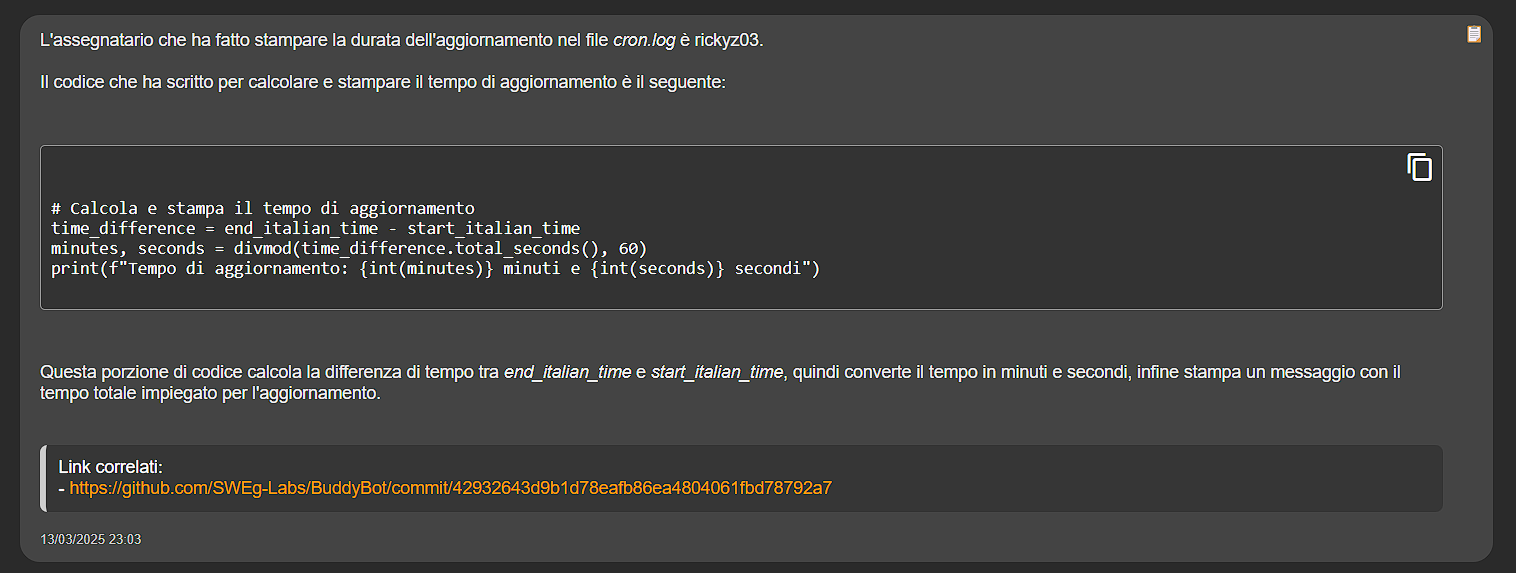
\includegraphics[width=.8\linewidth]{Risposta con snippet di codice.png}
        \caption{Risposta con snippet di codice}
        \label{fig:Risposta con snippet di codice}        
\end{figure}
\begin{figure}[h]
    \centering
        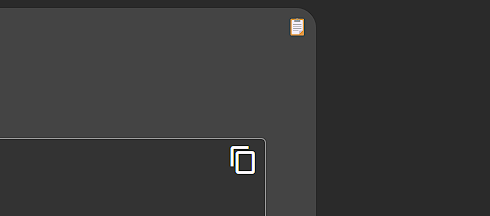
\includegraphics[width=.8\linewidth]{Pulsante di copia messaggio e pulsante di copia snippet di codice.png}
        \caption{Pulsante di copia messaggio (in alto) e pulsante di copia snippet di codice (in basso)}
        \label{fig:Pulsante di copia messaggio e pulsante di copia snippet di codice}        
\end{figure}
\begin{figure}[h]
    \centering
        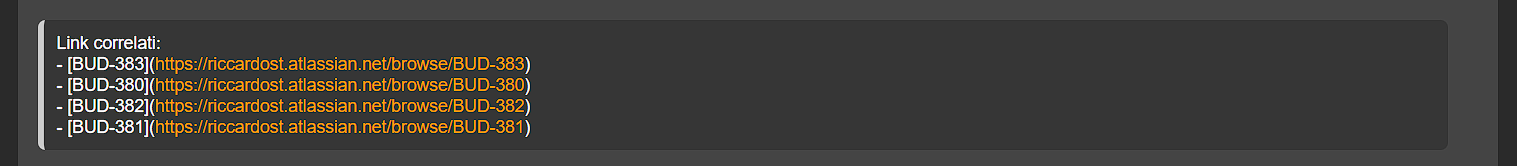
\includegraphics[width=.8\linewidth]{Riquadro dei link correlati.png}
        \caption{Riquadro dei link correlati}
        \label{fig:Riquadro dei link correlati}        
\end{figure}

\newpage


\subsection{Visualizzazione dello storico dei messaggi}
\label{subsec:visualizzazione_storico_messaggi}
Al primo accesso al chatbot, è possibile visualizzare la discussione vuota, senza alcun messaggio, come visibile in figura \bulref{fig:Discussione vuota}.\\
Una volta inviata la prima interrogazione, essa verrà visualizzata in alto a destra.
Una volta terminata l'elaborazione, la risposta del chatbot verrà visualizzata a sinistra, sotto il relativo messaggio.\\
Da qui in poi, ogni nuova interrogazione verrà visualizzata a destra, sotto la risposta precedente, mentre ogni risposta apparirà a sinistra, sotto la domanda corrispondente.\\
Sia le domande che le risposte sono corredate dalla data e dall'ora di invio, come visibile nelle figure \bulref{fig:Data e ora di invio domanda} e \bulref{fig:Data e ora di invio risposta}.\\
Quando si refresha la pagina, la discussione viene ripristinata, mostrando i 50 messaggi più recenti. È possibile visualizzare i messaggi precedenti tramite scroll: se si tenta di risalire ai messaggi dello storico non ancora caricati dal sistema, verrà visualizzata un'icona di una banana morsicata che rotea su se stessa che ne segnala il caricamento in corso, come si può vedere in figura \bulref{fig:Icona di caricamento dei messaggi precedenti}.\\
Terminata tale attesa, verranno visualizzati i 50 messaggi precedenti, e scrollando ancora si possono visualizzare i precedenti 50, e così via.
Se allo scroll l'icona di caricamento non appare, significa che si è giunti alla fine dello storico e non ci sono altri messaggi da visualizzare.\\
Una volta che ci si trova in alto nella conversazione, è possibile tornare velocemente in basso ai messaggi più recenti cliccando sull'apposito pulsante che appare in basso a destra, visibile in \bulref{fig:Pulsante per tornare ai messaggi recenti}.

\begin{figure}[h]
    \centering
        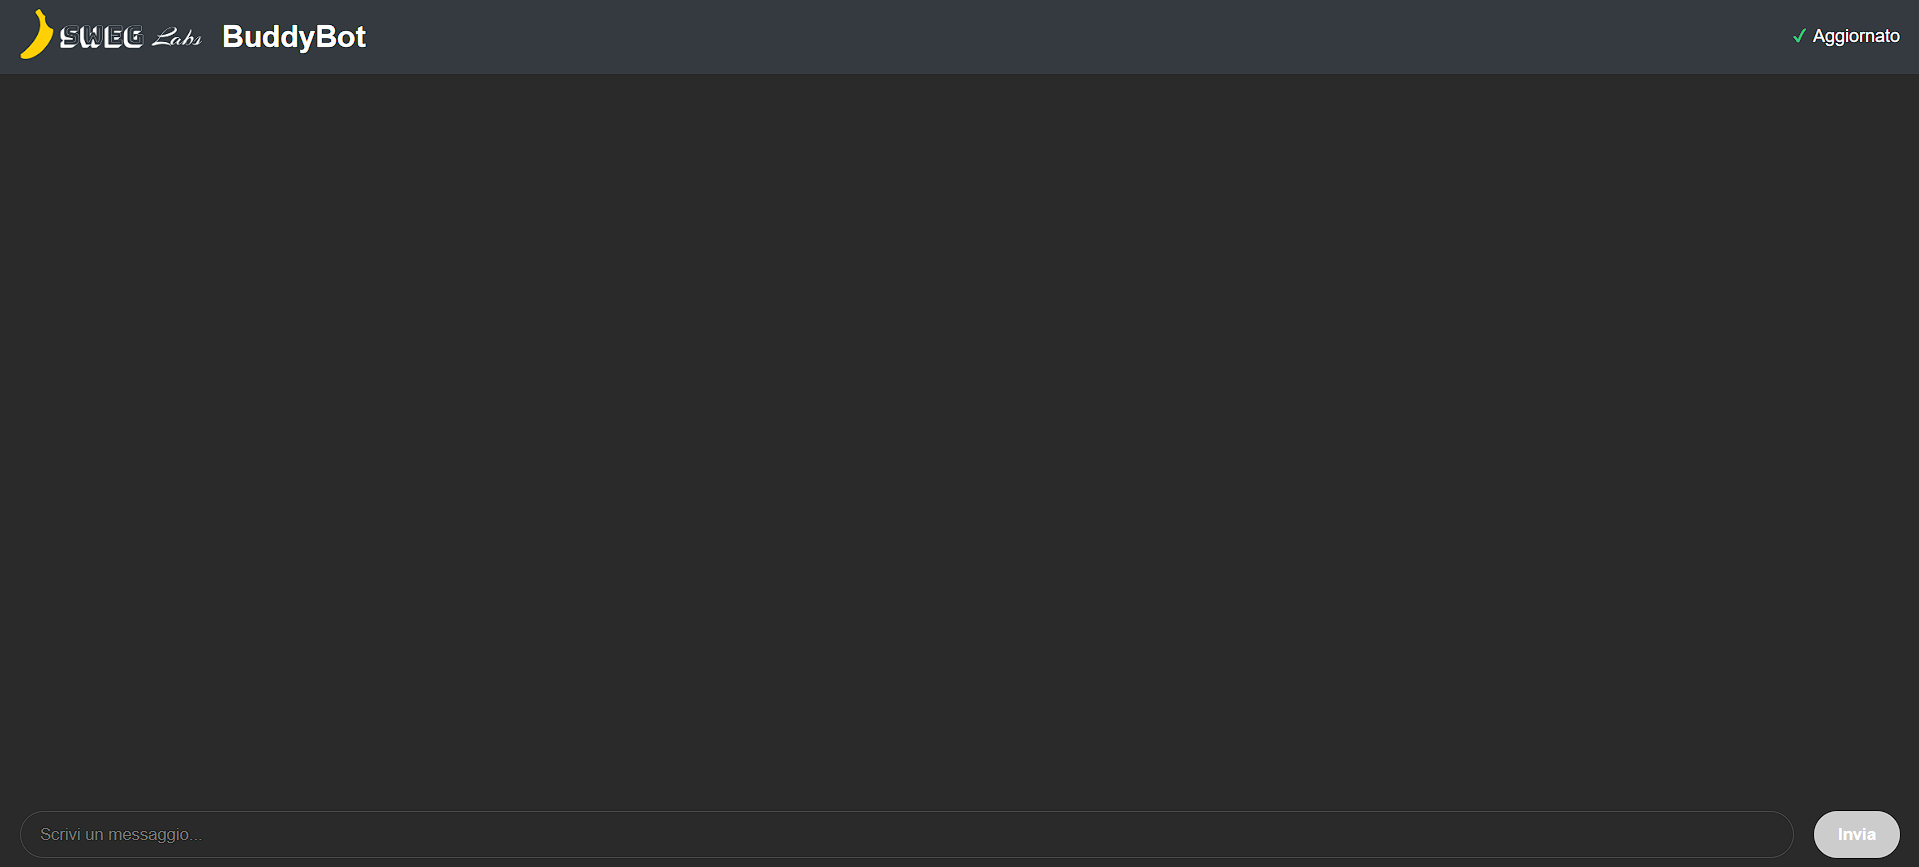
\includegraphics[width=.8\linewidth]{Schermata iniziale senza messaggi.png}
        \caption{Schermata iniziale vuota}
        \label{fig:Discussione vuota}        
\end{figure}
\begin{figure}[h]
    \centering
    \begin{minipage}[t]{.45\textwidth}
        \centering
        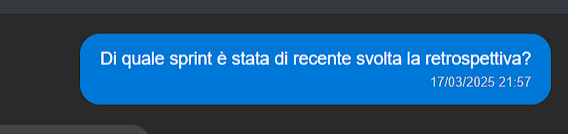
\includegraphics[height=2cm]{Data e ora invio messaggio - Utente.png}
        \caption{\centering Interrogazione con Data e Ora}
        \label{fig:Data e ora di invio domanda}
    \end{minipage}%
    \hfill
    \begin{minipage}[t]{.45\textwidth}
        \centering
        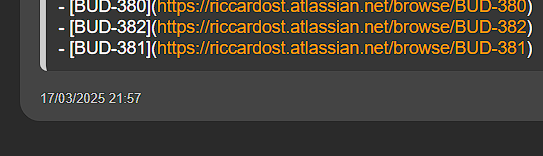
\includegraphics[height=2cm]{Data e ora di invio messaggio - Chatbot.png}
        \caption{\centering Messaggio di risposta con Data e Ora}
        \label{fig:Data e ora di invio risposta}
    \end{minipage}
\end{figure}
\begin{figure}[h]
    \centering
        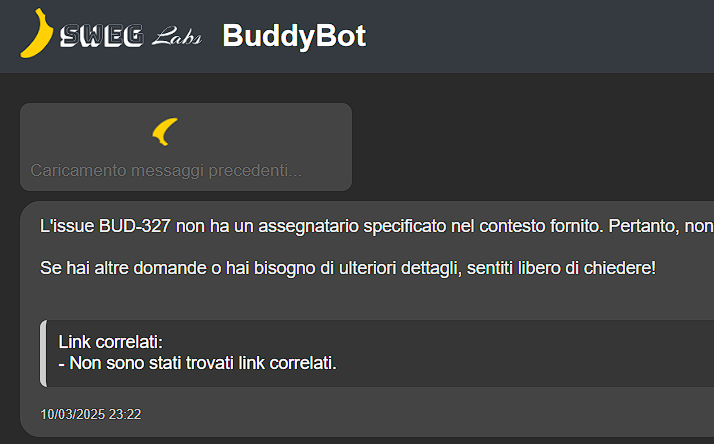
\includegraphics[height=6.5cm]{Icona di caricamento dei messaggi precedenti.png}
        \caption{Icona di caricamento dei messaggi precedenti}
        \label{fig:Icona di caricamento dei messaggi precedenti}
\end{figure}
\begin{figure}[h]
    \centering
        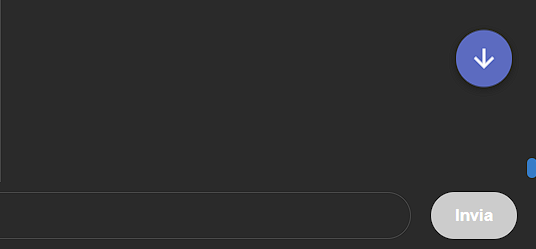
\includegraphics[width=.8\linewidth]{Pulsante per tornare ai messaggi recenti.png}
        \caption{Pulsante per tornare ai messaggi recenti}
        \label{fig:Pulsante per tornare ai messaggi recenti}
\end{figure}

\newpage


\subsection{Aggiornamento automatico dei documenti}
\label{subsec:aggiornamento_automatico_documenti}
Al fine di garantire che le informazioni fornite dal chatbot siano il più possibile attendibili, i documenti di contesto utilizzati per generare le risposte vengono aggiornati ogni 24 ore.
Tali aggiornamenti sono svolti in modo automatico, e non è dunque necessario alcun intervento di configurazione.
È possibile che, nel momento in cui si pone una domanda, l'aggiornamento automatico dei documenti sia in corso, e quindi potrebbe avvenire un errore nella generazione della risposta. In tal caso, è consigliabile attendere qualche minuto e riprovare.
In alto a destra è presente un badge di segnalazione che indica l'esito dell'ultimo aggiornamento:
\begin{itemize}
    \item Se il badge presenta una spunta verde con accanto la scritta \emph{Aggiornato}, come visibile in figura \bulref{fig:Aggiornamento avvenuto con successo}, significa che l'ultimo aggiornamento è avvenuto con successo, e le risposte fornite
    dal chatbot sono aggiornate ai documenti non più vecchi di 24 ore;
    \item Se il badge presenta una X rossa con accanto la scritta \emph{Non aggiornato}, come visibile in figura \bulref{fig:Aggiornamento fallito}, significa che l'ultimo aggiornamento è fallito, e le risposte fornite dal chatbot potrebbero
    non essere aggiornate ai documenti più recenti;
    \item Se il badge presenta un segnale di pericolo con accanto la scritta \emph{Errore}, come visibile in figura \bulref{fig:Errore nel recupero dell'esito dell'ultimo aggiornamento}, significa che non è stato possibile recuperare l'esito dell'ultimo aggiornamento, e, dunque, non è possibile sapere se le risposte fornite dal chatbot sono aggiornate ai documenti più recenti o meno.
\end{itemize}

\begin{figure}[h]
    \centering
        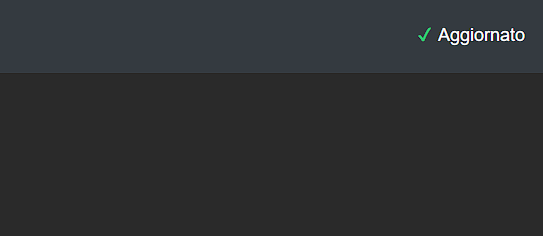
\includegraphics[width=.8\linewidth]{Badge - Aggiornamento avvenuto con successo.png}
        \caption{Badge di aggiornamento avvenuto con successo}
        \label{fig:Aggiornamento avvenuto con successo}        
\end{figure}

\newpage

\begin{figure}[h]
    \centering
        
\includegraphics[width=.8\linewidth]{Badge - Aggiornamento fallito.png}
        \caption{Badge di aggiornamento fallito}
        \label{fig:Aggiornamento fallito}
\end{figure}

\begin{figure}[h]
    \centering
        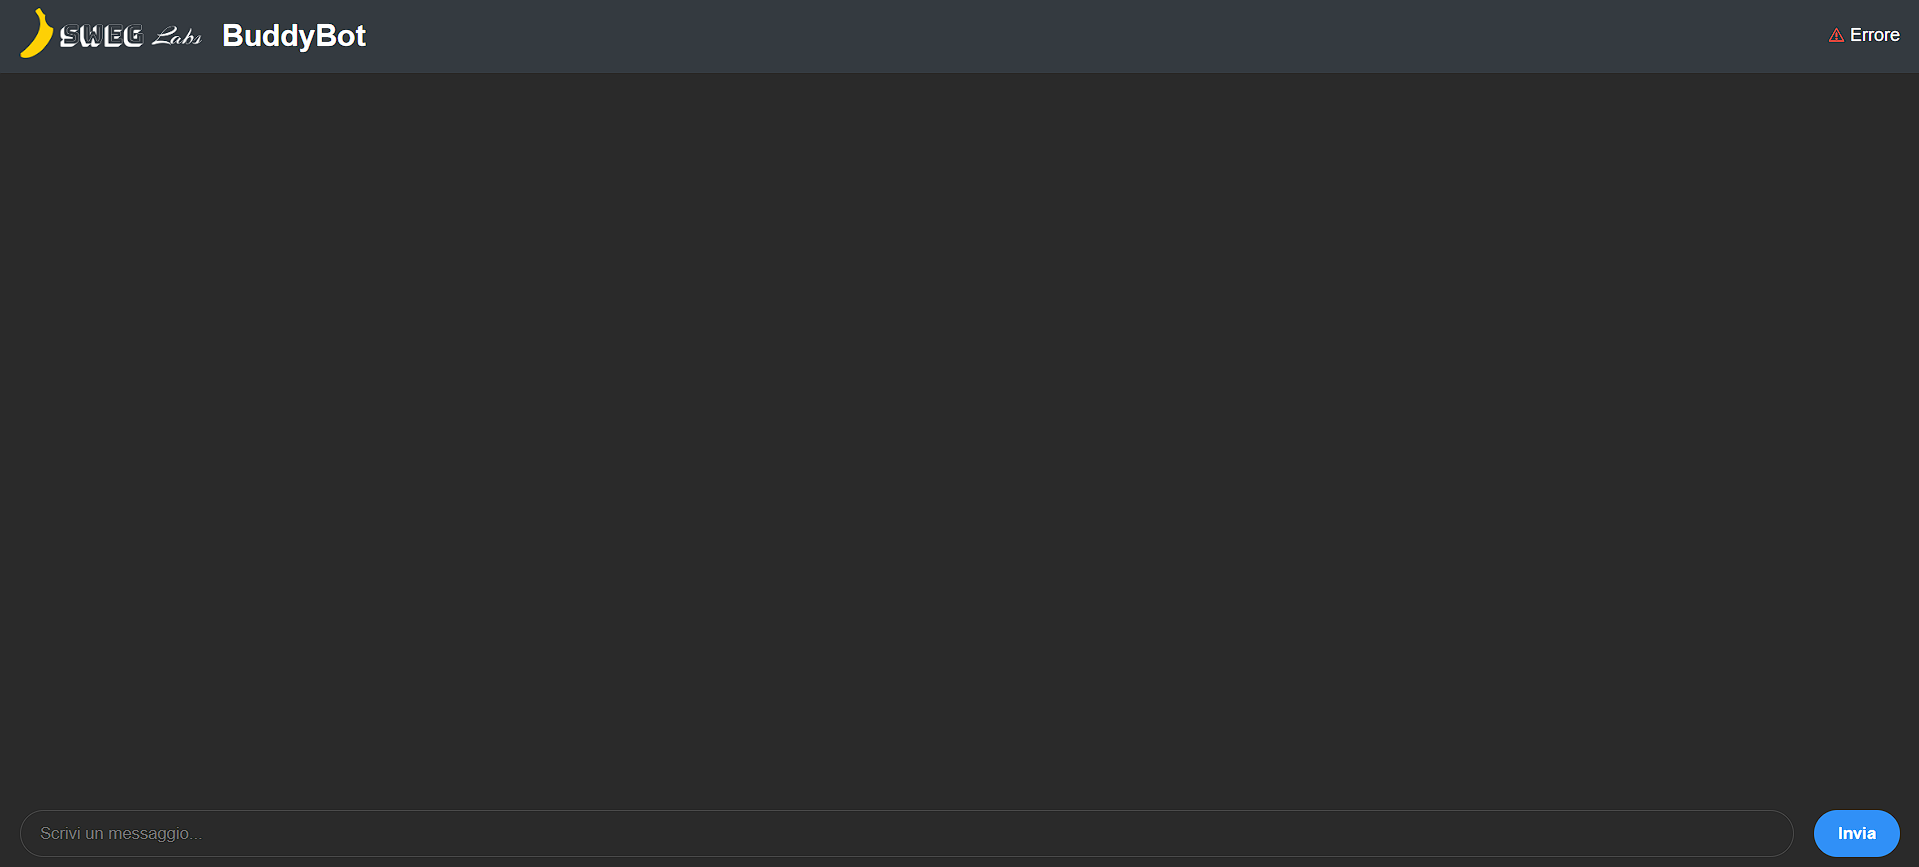
\includegraphics[width=.8\linewidth]{Badge - Errore recupero esito aggiornamento.png}
        \caption{Badge di errore nel recupero dell'esito dell'ultimo aggiornamento}
        \label{fig:Errore nel recupero dell'esito dell'ultimo aggiornamento}
\end{figure}



\newpage

\subsection{Possibili errori}
\label{subsec:possibili_errori}

Durante l'utilizzo del chatbot è possibile che si verifichino alcuni errori. Lo scopo di questa sezione è presentare alcune casistiche non desiderate e fornire una guida per ripristinare il corretto funzionamento.


\subsubsection{Errore nel recupero dello storico dei messaggi}

\begin{figure}[h]
    \centering
        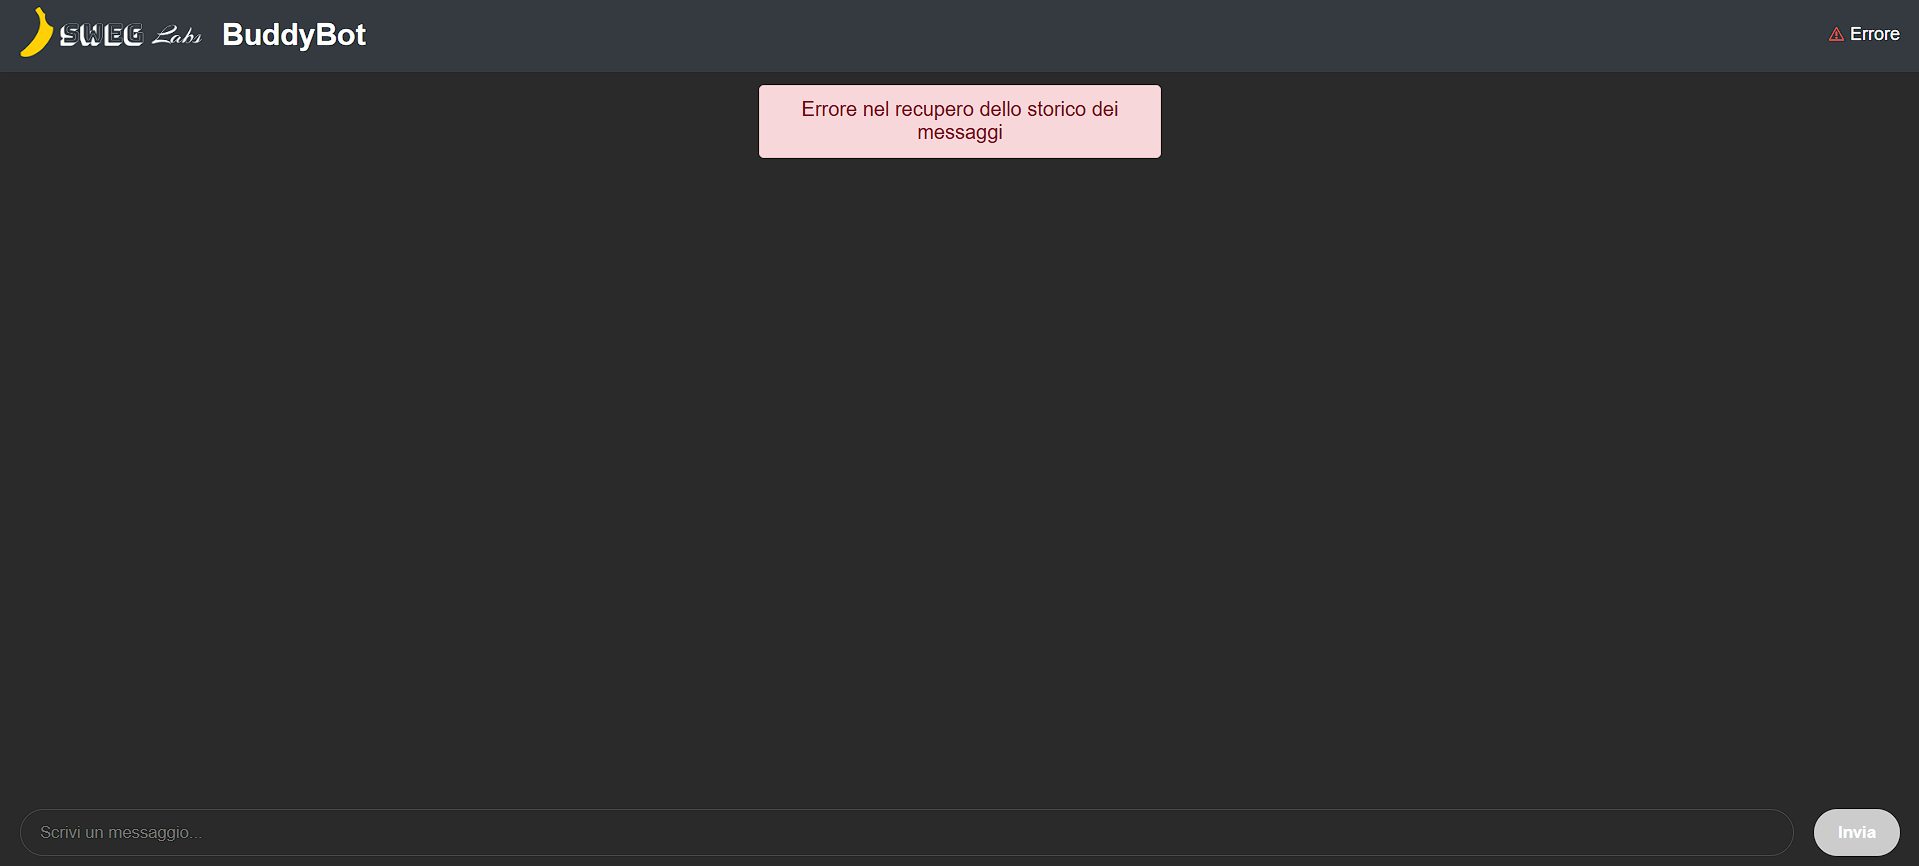
\includegraphics[width=.8\linewidth]{Errore - Recupero storico messaggi dal database.png}
        \caption{Errore nel recupero dello storico dei messaggi}
        \label{fig:Errore nel recupero dello storico dei messaggi}
\end{figure}

Nel caso non sia possibile recuperare i messaggi delle precedenti conversazioni, verrà mostrato in alto un apposito riquadro che comunica il problema, come visibile in figura \bulref{fig:Errore nel recupero dello storico dei messaggi}. E' probabile che ciò sia dovuto ad un problema con il \emph{database relazionale}\textsubscript{\textbf{\textit{G}}} \emph{Postgres}\textsubscript{\textbf{\textit{G}}}; il consiglio dunque è di recarsi su \emph{Docker Desktop}\textsubscript{\textbf{\textit{G}}} e di controllare se il \emph{container}\textsubscript{\textbf{\textit{G}}} dedicato a \emph{Postgres} è acceso, ed eventualmente riavviarlo. Nel caso ciò non sia sufficiente, controllare allora lo stato del container di \emph{backend}\textsubscript{\textbf{\textit{G}}}, poichè anch'esso ha un ruolo fondamentale nella funzionalità di recupero dei vecchi messaggi, e provare dunque a riavviare anch'esso.


\subsubsection{Errore nella generazione della risposta}

\begin{figure}[h]
    \centering
        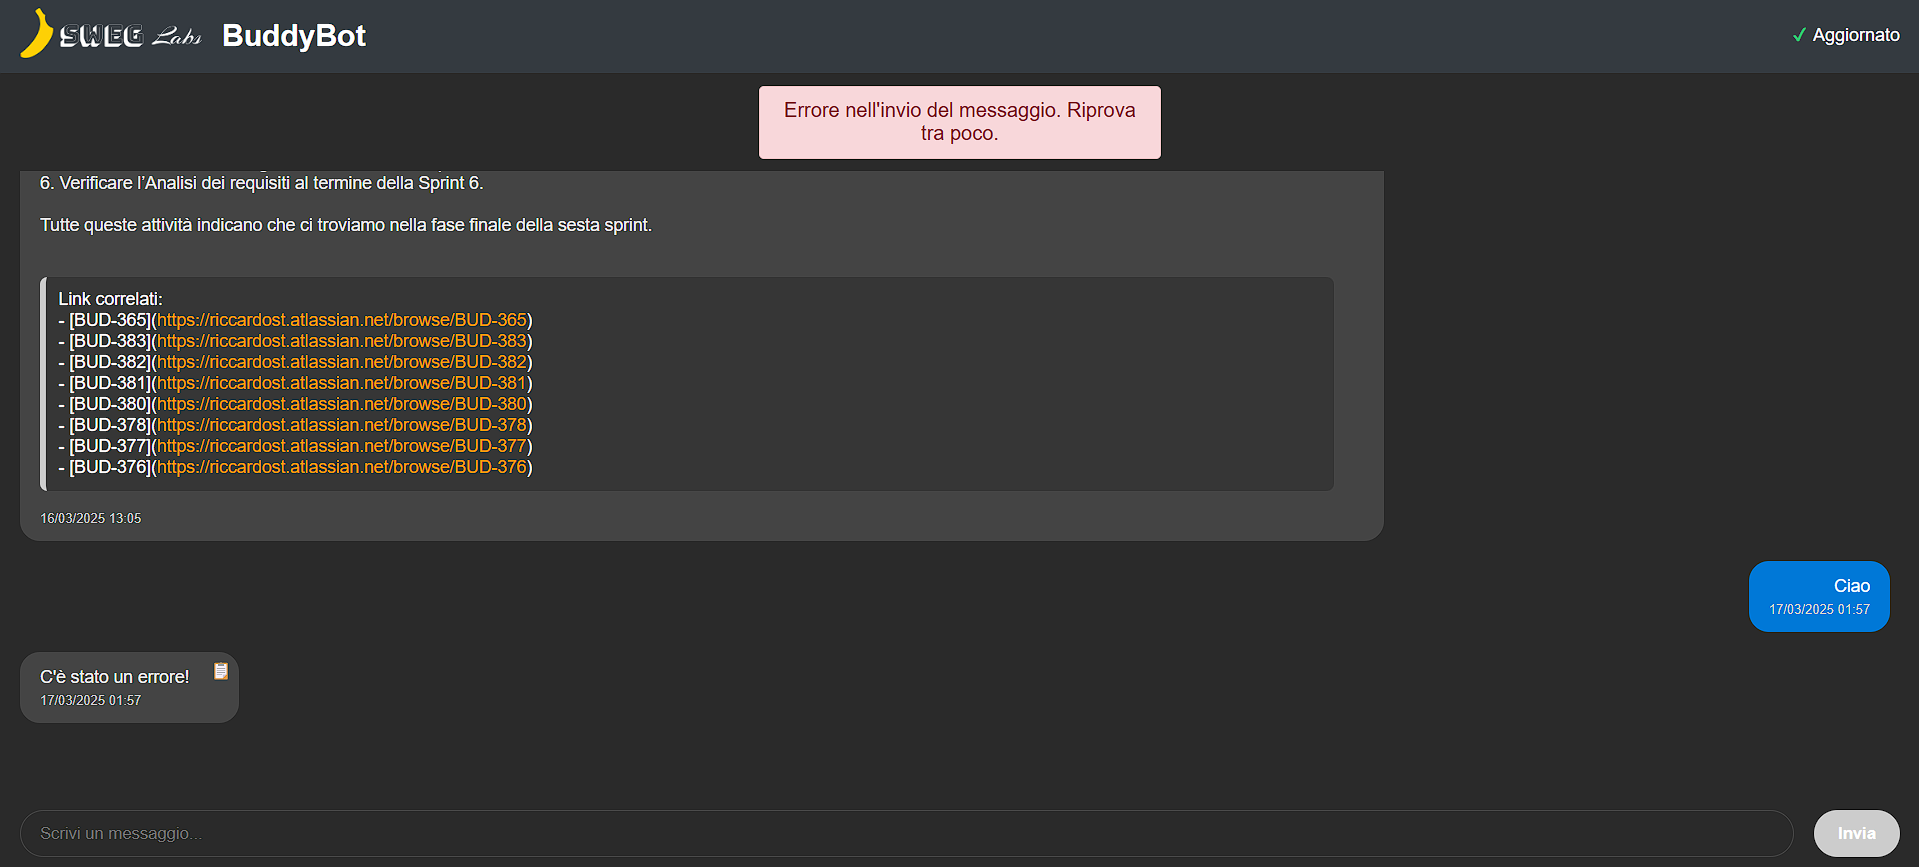
\includegraphics[width=.8\linewidth]{Errore - Generazione della risposta.png}
        \caption{Errore nella generazione della risposta}
        \label{fig:Errore nella generazione della risposta}
\end{figure}

Nel caso avvenga un errore nella generazione della risposta, verrà ricevuto un messaggio di errore e, in alto, apparirà per pochi secondi un avviso che invita a riprovare più tardi, come visibile in figura \bulref{fig:Errore nella generazione della risposta}. L'errore può essere dovuto principalmente a tre motivi:
\begin{itemize}
    \item \textbf{Scarsa connessione a internet, tale per cui non è stato possibile contattare l'\emph{LLM}\textsubscript{\textbf{\textit{G}}}}: in tal caso, il consiglio è di provare a disconnettersi e riconnettersi e poi riprovare;
    \item \textbf{Problemi con il container di backend}: in tal caso, il consiglio è provare a spegnerlo e riaccenderlo in Docker Desktop;
    \item \textbf{Contemporaneità tra l'aggiornamento automatico dei documenti e l'invio di una domanda}: in tal caso, il consiglio è di attendere qualche minuto e poi riprovare.
\end{itemize}



\subsubsection{Errore nel recupero del link dei file correlati alla risposta}

\begin{figure}[h]
    \centering
        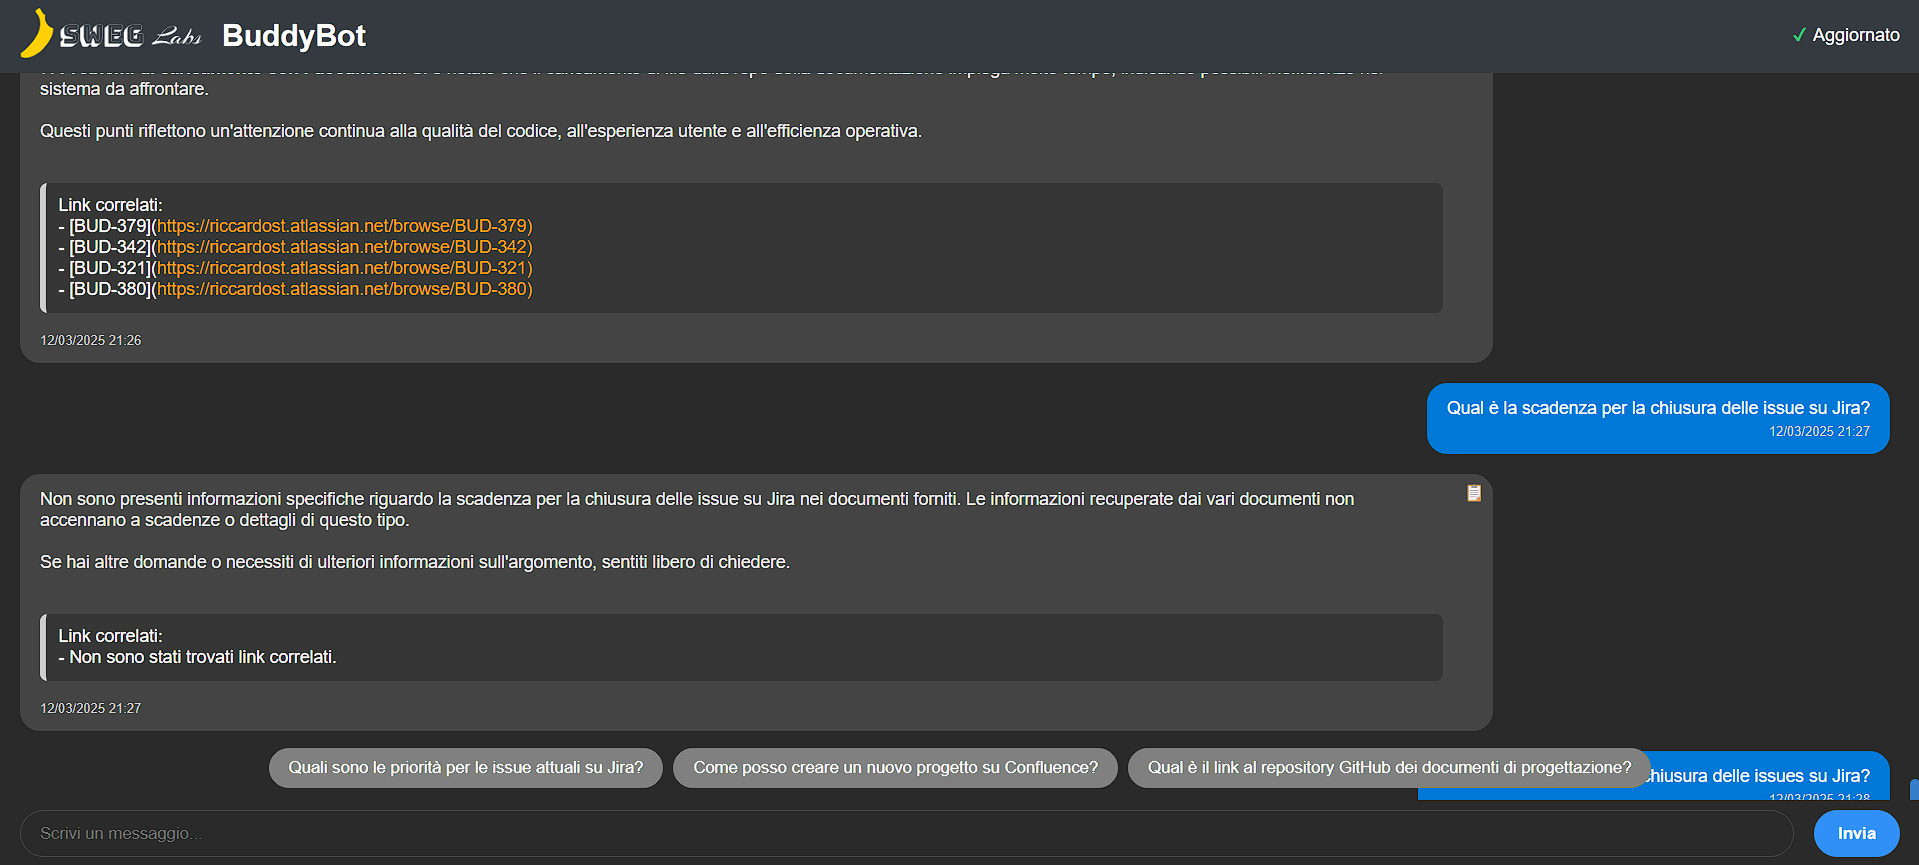
\includegraphics[width=.8\linewidth]{Errore - Non sono stati trovati link correlati.png}
        \caption{Errore nel recupero del link dei file correlati alla risposta}
        \label{fig:Errore nel recupero del link dei file correlati alla risposta}
\end{figure}

Nel caso avvenga un errore nel recupero dei link correlati alla risposta appena generata, verrà mostrato il consueto riquadro alla fine del messaggio, ma contenente, invece che i link, una frase descrittiva del problema, come visibile in figura \bulref{fig:Errore nel recupero del link dei file correlati alla risposta}. Siccome la risposta è stata generata normalmente, il motivo per la mancata visualizzazione dei link è da ricercare nella correttezza della domanda, che probabilmente non rispetta le istruzioni fornite nella sezione \S\bulref{subsec:cosa_come_chiedere} di questo documento. Ad esempio, in figura è stata posta una domanda che chiede quali sono le fasi del ciclo di vita di un ticket su \emph{Jira}\textsubscript{\textbf{\textit{G}}}, la quale viola il punto 11 della suddetta sezione: come si può notare, la risposta viene comunque generata, ma non è attendibile, poichè infatti non è stata citata nessuna fonte a suo sostegno. Fortunatamente, rispettando assiduamente la guida su cosa chiedere e come chiederlo, l'errore nel recupero dei link correlati alla risposta non dovrebbe mai avvenire.


\subsubsection{Visualizzazione errore nel recupero della data e ora di invio del messaggio}

\begin{figure}[h]
    \centering
        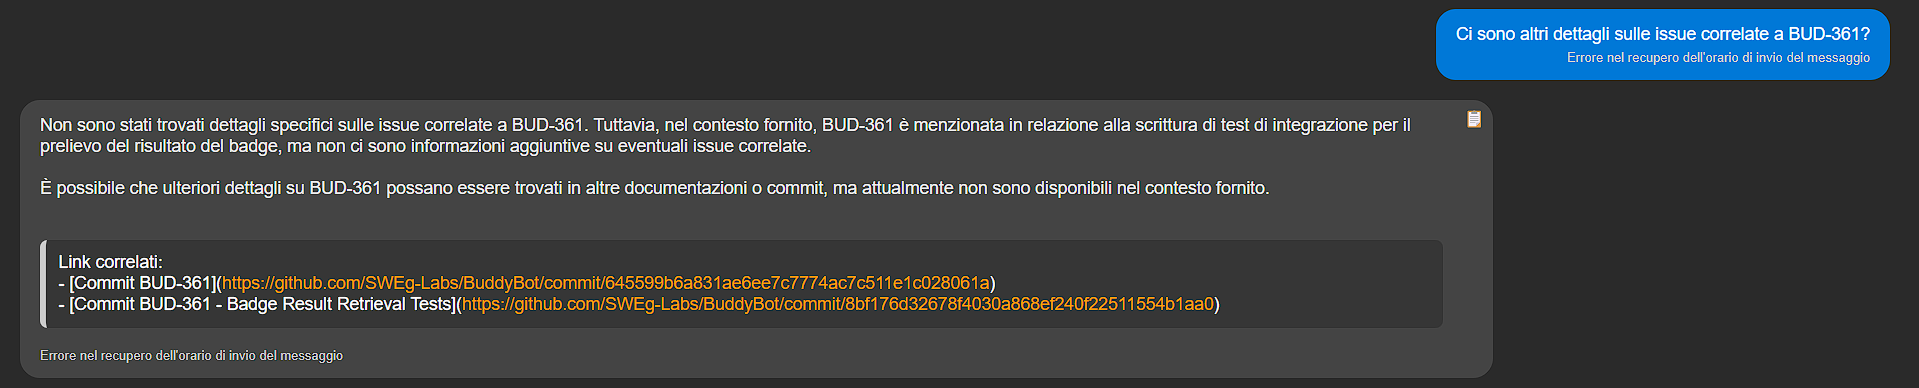
\includegraphics[width=.8\linewidth]{Errore - Recupero data e ora di invio del messaggio.png}
        \caption{Errore nel recupero della data e ora di invio del messaggio}
        \label{fig:Errore nel recupero della data e ora di invio del messaggio}
\end{figure}

Nel caso non sia possibile recuperare la data e l'ora di invio del messaggio, verrà mostrata al loro posto una scritta segnalante l'errore, come visibile in figura \bulref{fig:Errore nel recupero della data e ora di invio del messaggio}. E' probabile che ciò sia dovuto ad un problema con il \emph{database relazionale}\textsubscript{\textbf{\textit{G}}} \emph{Postgres}\textsubscript{\textbf{\textit{G}}}; il consiglio dunque è di recarsi su \emph{Docker Desktop} e di controllare se il \emph{container} dedicato a \emph{Postgres} è acceso, ed eventualmente riavviarlo. Nel caso ciò non sia sufficiente, controllare allora lo stato del container di backend, poichè anch'esso ha un ruolo fondamentale nella funzionalità di recupero della data e ora di invio del messaggio, e provare dunque a riavviare anch'esso.


\subsubsection{Errore nella generazione delle domande per proseguire la conversazione}

\begin{figure}[h]
    \centering
        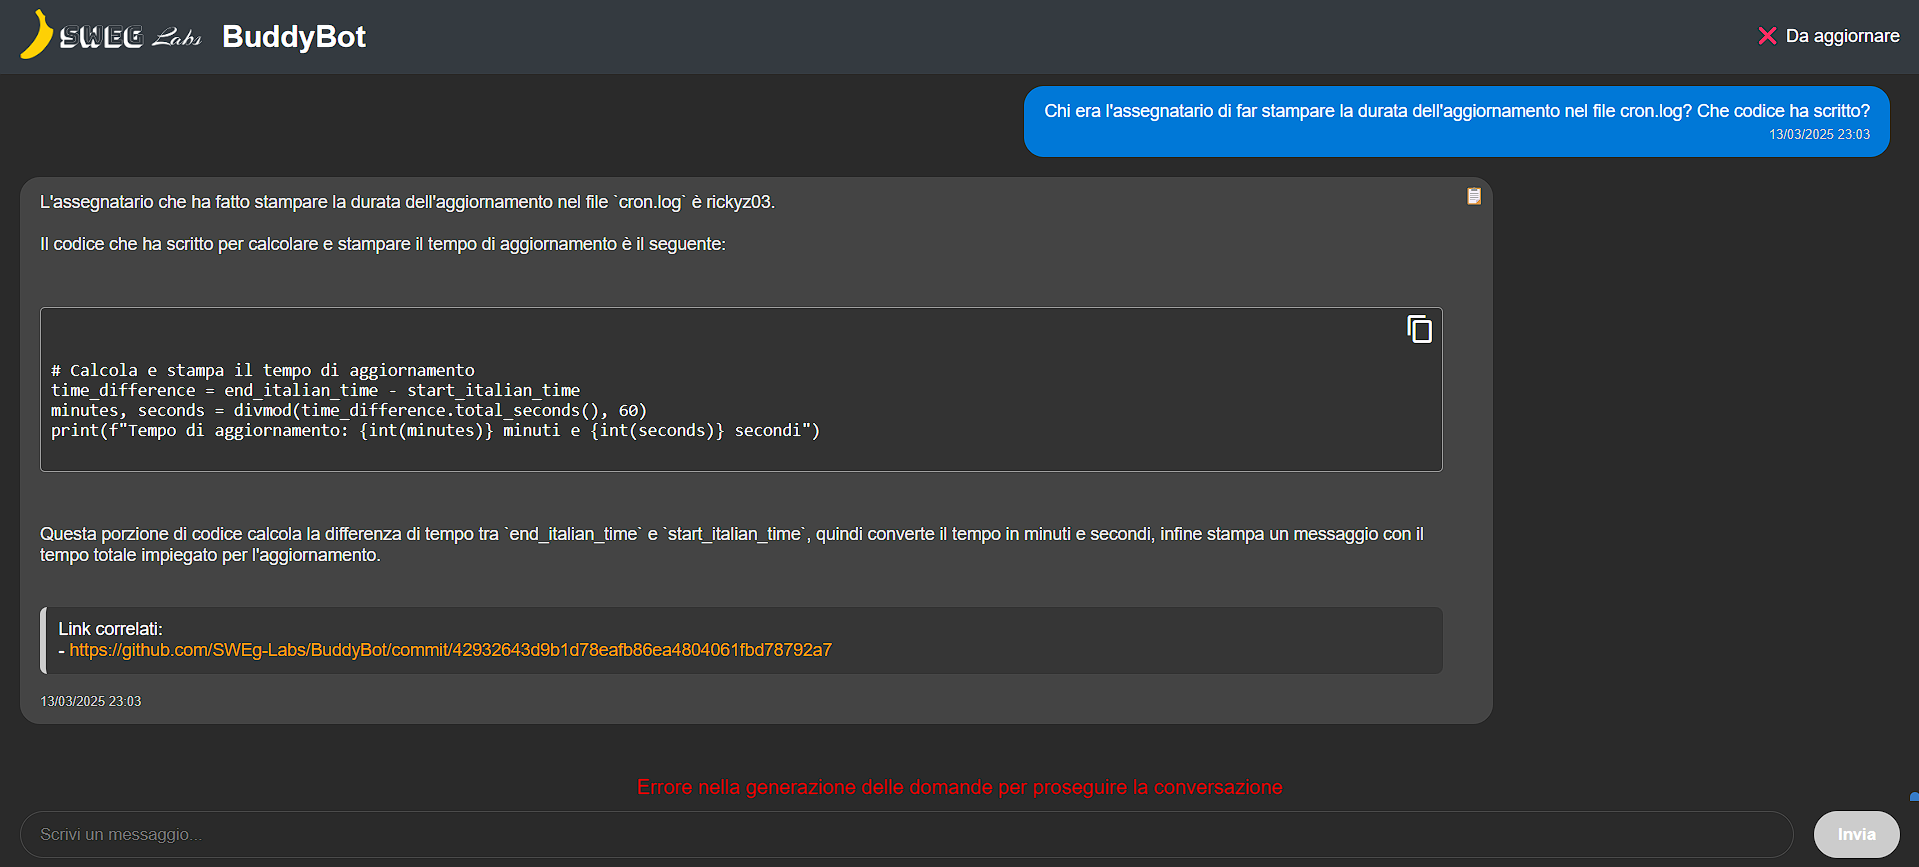
\includegraphics[width=.8\linewidth]{Errore - Generazione di domande per proseguire la conversazione.png}
        \caption{Errore nella generazione delle domande per proseguire la conversazione}
        \label{fig:Errore nella generazione delle domande per proseguire la conversazione}
\end{figure}

Nel caso avvenga un errore nella generazione delle domande suggerite per proseguire la conversazione, verrà mostrata una scritta rossa comunicante il problema sopra alla barra di input, come visibile in figura \bulref{fig:Errore nella generazione delle domande per proseguire la conversazione}. L'errore può essere dovuto principalmente a due motivi:
\begin{itemize}
    \item \textbf{Scarsa connessione a internet, tale per cui non è stato possibile contattare l'\emph{LLM}}: in tal caso, il consiglio è di provare a disconnettersi e riconnettersi e poi riprovare;
    \item \textbf{Problemi con il container di backend}: in tal caso, il consiglio è provare a spegnerlo e riaccenderlo in Docker Desktop.
\end{itemize}


\subsubsection{Visualizzazione di un badge che segnala un errore nell'ultimo aggiornamento del database vettoriale}

\begin{figure}[h]
    \centering
        
\includegraphics[width=.8\linewidth]{Badge - Aggiornamento fallito.png}
        \caption{Badge di aggiornamento fallito}
        \label{fig:Badge di aggiornamento fallito}
\end{figure}

Come descritto nella sezione \S\bulref{subsec:aggiornamento_automatico_documenti}, nel caso l'ultimo aggiornamento del database vettoriale sia fallito, verrà mostrato in alto a destra un badge di segnalazione che indica il fallimento, come visibile in figura \bulref{fig:Aggiornamento fallito}. E' probabile che ciò sia dovuto ad un problema con il \emph{database vettoriale} \emph{Chroma}\textsubscript{\textbf{\textit{G}}}; il consiglio dunque è di recarsi su \emph{Docker Desktop} e di controllare se il \emph{container} dedicato a \emph{Chroma} è acceso, ed eventualmente riavviarlo. Nel caso ciò non sia sufficiente, controllare allora lo stato del container di backend, poichè anch'esso ha un ruolo fondamentale nella funzionalità di aggiornamento automatico dei documenti, e provare dunque a riavviare anch'esso.


\subsubsection{Visualizzazione errore nel recupero dell'esito dell'ultimo aggiornamento del database vettoriale}

\begin{figure}[h]
    \centering
        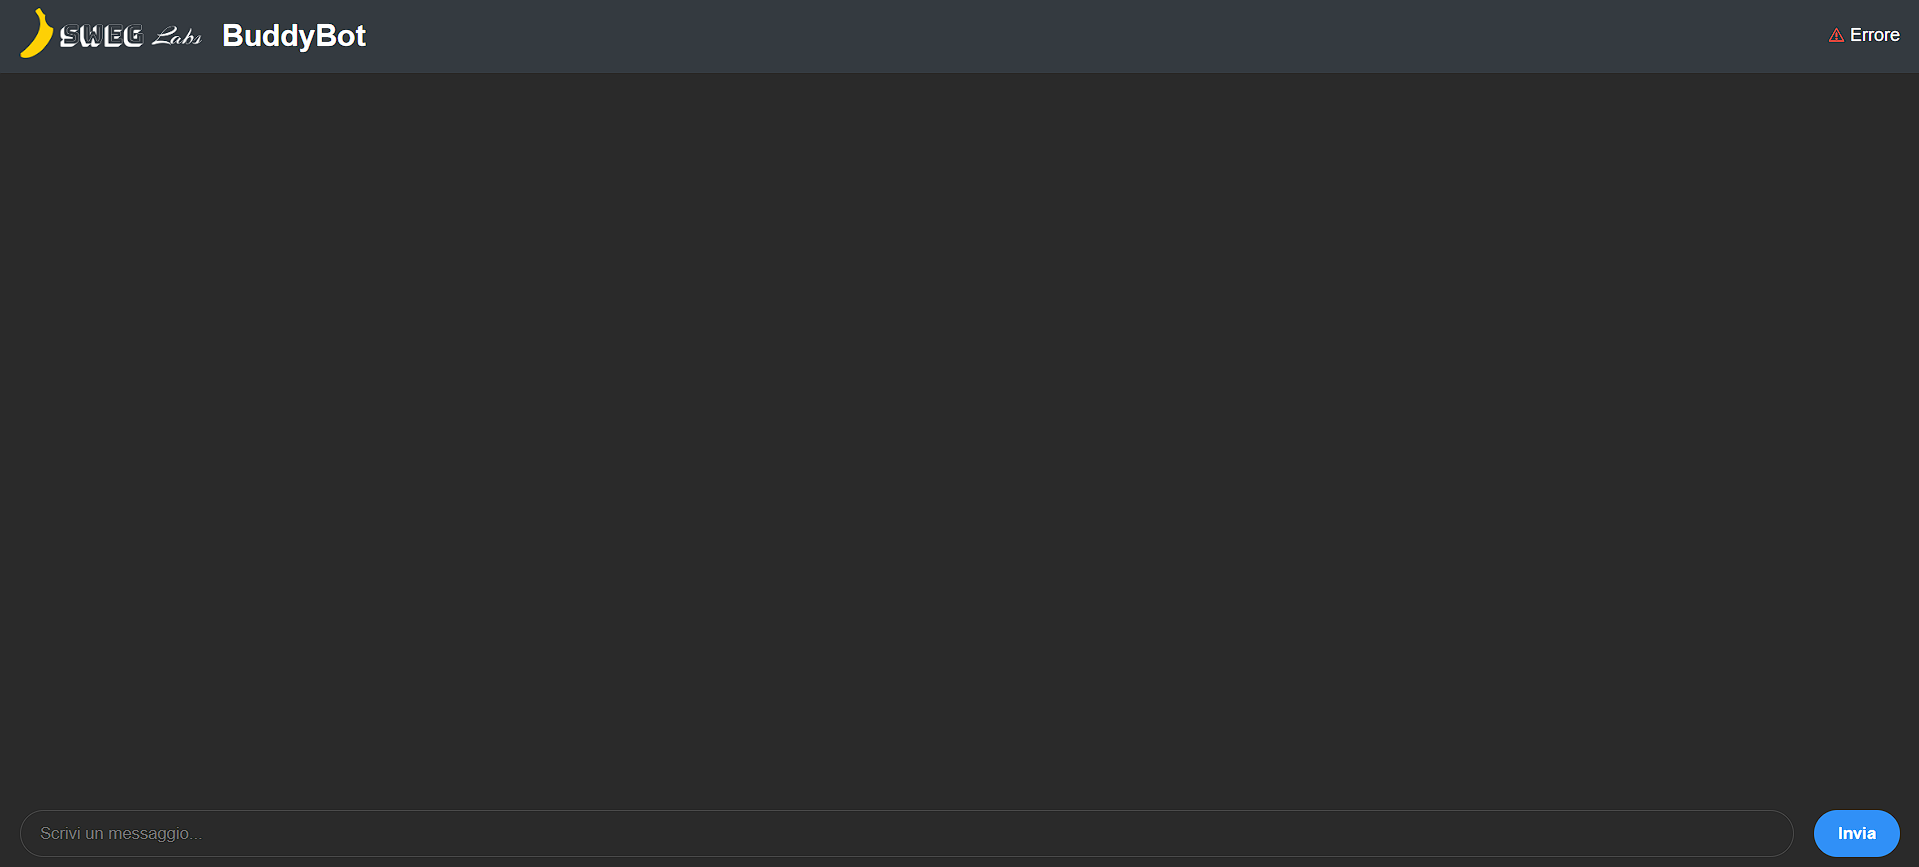
\includegraphics[width=.8\linewidth]{Badge - Errore recupero esito aggiornamento.png}
        \caption{Badge di errore nel recupero dell'esito dell'ultimo aggiornamento}
        \label{fig:Badge di errore nel recupero dell'esito dell'ultimo aggiornamento}
\end{figure}

Come descritto nella sezione \S\bulref{subsec:aggiornamento_automatico_documenti}, nel caso non sia possibile recuperare l'esito dell'ultimo aggiornamento del database vettoriale, verrà mostrato in alto a destra un badge di segnalazione che indica l'errore, come visibile in figura \bulref{fig:Badge di errore nel recupero dell'esito dell'ultimo aggiornamento}. E' probabile che ciò sia dovuto ad un problema con il \emph{database relazionale} \emph{Postgres}; il consiglio dunque è di recarsi su \emph{Docker Desktop} e di controllare se il \emph{container} dedicato a \emph{Postgres} è acceso, ed eventualmente riavviarlo. Nel caso ciò non sia sufficiente, controllare allora lo stato del container di backend, poichè anch'esso ha un ruolo fondamentale nella funzionalità di recupero dell'esito dell'ultimo aggiornamento del database vettoriale, e provare dunque a riavviare anch'esso.


\subsubsection{Visualizzazione errore nel recupero dei messaggi precedenti allo scroll}

\begin{figure}[h]
    \centering
        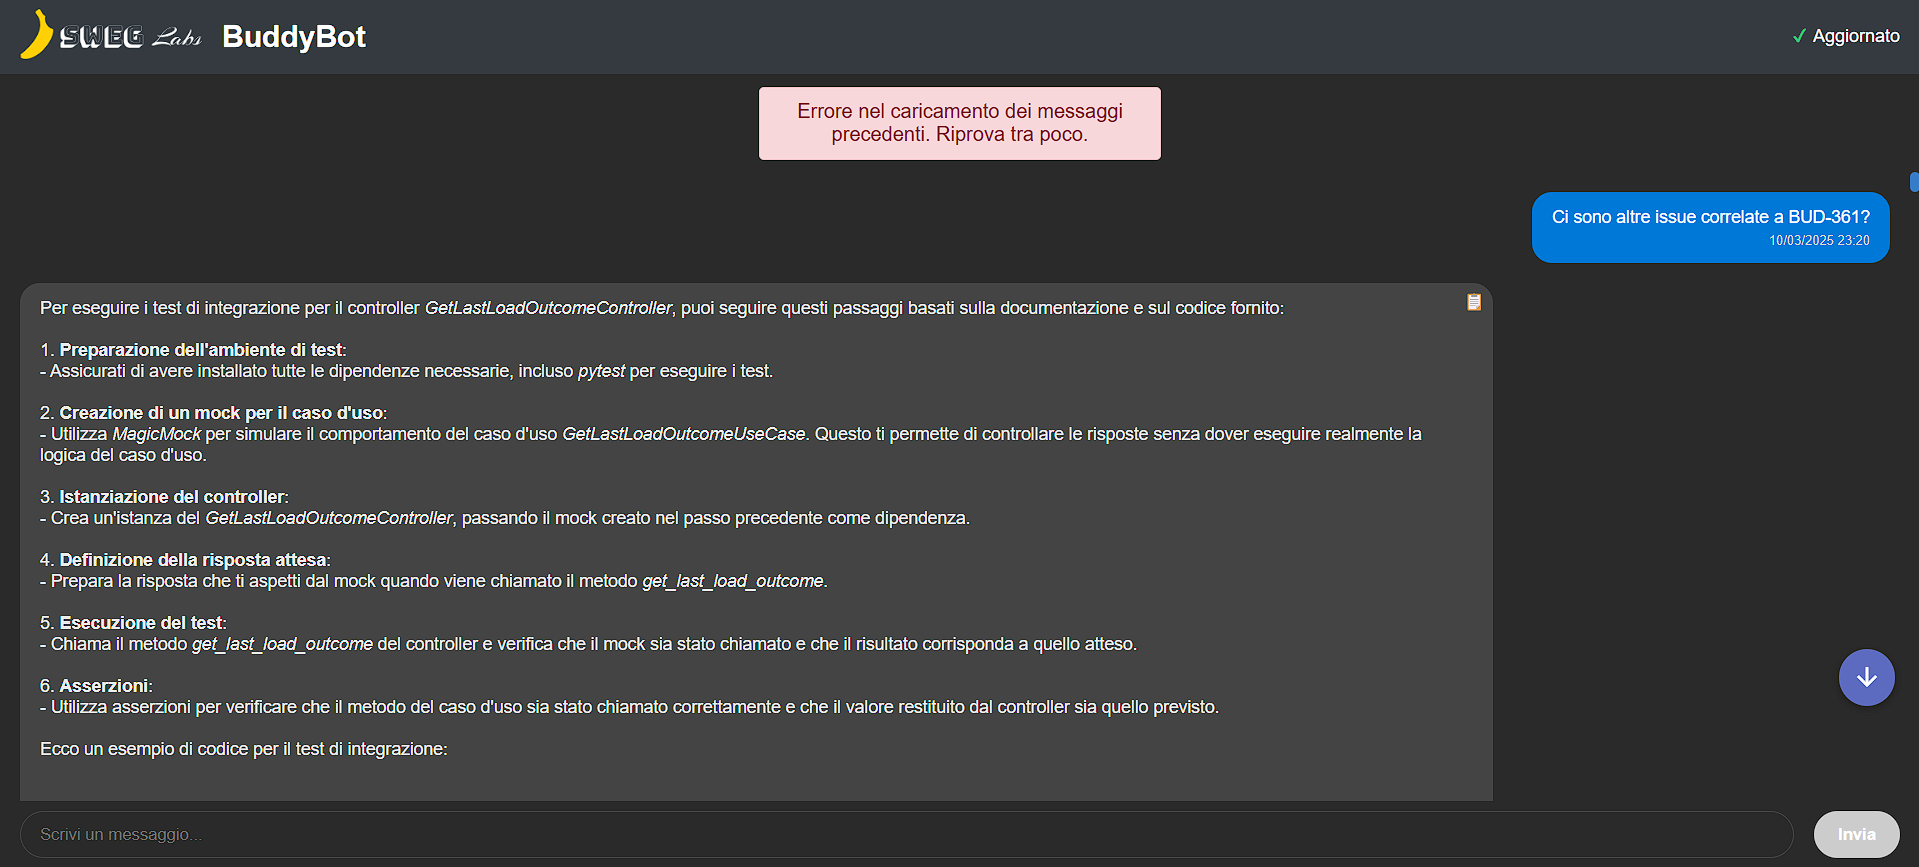
\includegraphics[width=.8\linewidth]{Errore - Recupero messaggi precedenti dal database.png}
        \caption{Errore nel recupero dei messaggi precedenti allo scroll}
        \label{fig:Errore nel recupero dei messaggi precedenti allo scroll}
\end{figure}

Nel caso non sia possibile recuperare i messaggi delle precedenti conversazioni allo scroll dello schermo, verrà mostrato in corrispondenza del confine superiore della chat, per pochi secondi, un avviso che invita a riprovare più tardi, come visibile in figura \bulref{fig:Errore nel recupero dei messaggi precedenti allo scroll}. E' probabile che ciò sia dovuto ad un problema con il \emph{database relazionale} \emph{Postgres}; il consiglio dunque è di recarsi su \emph{Docker Desktop} e di controllare se il \emph{container} dedicato a \emph{Postgres} è acceso, ed eventualmente riavviarlo. Nel caso ciò non sia sufficiente, controllare allora lo stato del container di backend, poichè anch'esso ha un ruolo fondamentale nella funzionalità di recupero dei vecchi messaggi, e provare dunque a riavviare anch'esso.
